%!TEX root = ../../../thesis.tex
\begin{figure}
    \centering
    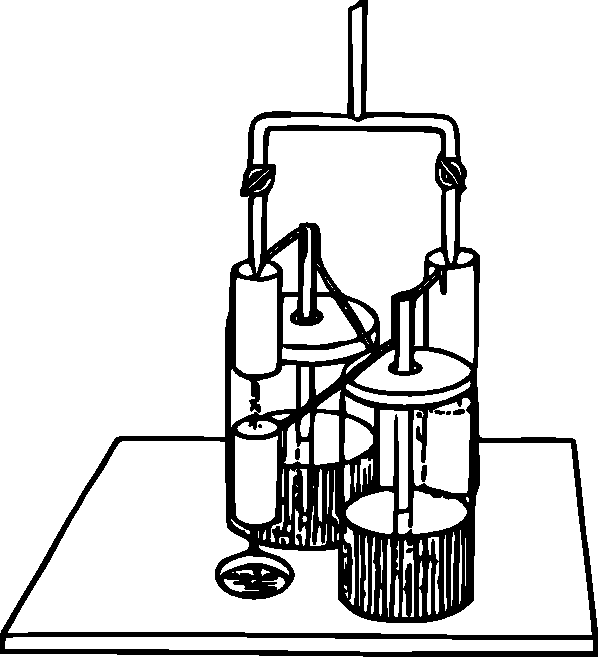
\includegraphics[width=0.5\textwidth]{content/appendices/chargedWaterDrops/graphics/Figure_Drawing_KelvinWaterDripper_OriginalDevice}
    \caption{Drawing of Lord Kelvin's electrostatic generator~\cite{Thomson1867a}.}
    \label{Figure_Drawing_KelvinWaterDripper_OriginalDevice}
\end{figure}
In 1867 William Thomson (Lord Kelvin) described an apparatus that could generate electrostatic charge using drops of water~\cite{Thomson1867}.
\Cref{Figure_Drawing_KelvinWaterDripper_OriginalDevice} shows original artwork of the device from that paper.
It works by inducing charge onto drops of water before they detach from the source of the drips.
This device was the starting point of investigation into the use of charged water drops to generate electrical power.


\section{Generating Charge}

  \begin{figure}
      \centering
      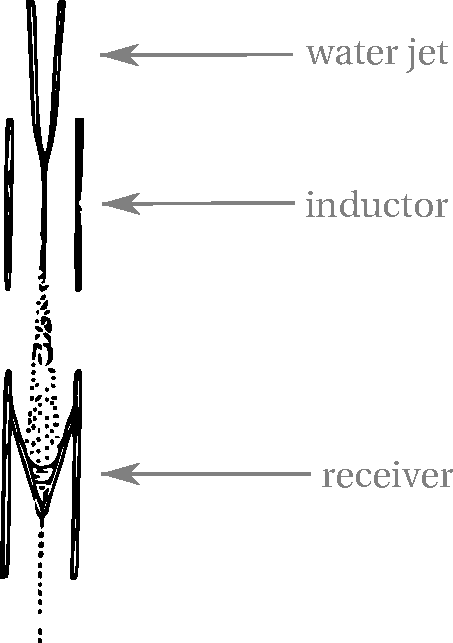
\includegraphics[height=0.25\textheight]{content/appendices/chargedWaterDrops/graphics/Figure_Drawing_KelvinWaterDripper_ChargingMechanism}
      \caption{Drawing of the charging mechanism for Lord Kelvin's electrostatic
  generator}
      \label{Figure_Drawing_KelvinWaterDripper_ChargingMechanism}
  \end{figure}
  Figure \ref{Figure_Drawing_KelvinWaterDripper_ChargingMechanism} shows charge generating mechanism of Lord Kelvin's electrostatic generator.
  This mechanism is comprised of three main components:
  \begin{enumerate}
  \item a jet of water which breaks into droplets,
  \item an inducting ring surrounding the area where the jet breaks up,
  \item a receiver where the charged droplets are collected.
  \end{enumerate}
  \begin{figure}
      \centering
      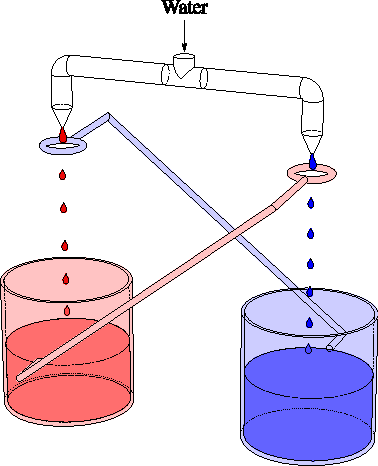
\includegraphics{content/appendices/chargedWaterDrops/graphics/DripperOut}
      \caption{\label{Fig_Diagram_KelvinWaterDripper}Simplified diagram of Lord Kelvin's water dropper configuration}
  \end{figure}
  A diagram showing a variation of that design with both sides present is shown as \cref{Fig_Diagram_KelvinWaterDripper}.
  The polarity of each receiver and induction ring is represented by its colour.
  Equal and opposite charge is accumulated in the receivers below the nozzles.
  The receivers are electrically isolated from each other, but are connected to the induction rings of the opposite side.
  The induction rings push charge away from the drop as it forms on the positive side, and pulls charge onto drops forming on the negative side.
  Gravity then pulls the drops down into the receivers below.
  Because the receiver and the drip both have the same polarity electric field, they repel each other.
  The drop, because of gravity and the height it falls from, is doing work as it falls into the receiver as the integral of the electrostatic force over the distance it travels.
  The result of that work is an increase in static charge held by the receiver, measured as voltage.


\section{Optimising output}

  Summer research student Jonathon McMullen assembled a test-rig to recreate the experiment.
  Once constructed, another summer research student, Wayne Crump, and myself took measurements.
  Then we sought to optimise the design in the hopes that is may be suitable as an energy harvester.


  \subsection*{Drop volume and frequency}

    The first optimisation question was ``is it better to have many small or fewer but larger drops?''.
    A simplified experiment was made with the help of Wayne Crump.
    We aimed to remove as many variables from the experiment that was previously performed by Jonathan McMullen.
    By doing so we hoped to isolate the effect of varying drop size, induction voltage, and flow rate, had on output power.


  \subsubsection*{Experimental setup}

  \begin{figure}[ht]
        \centering
        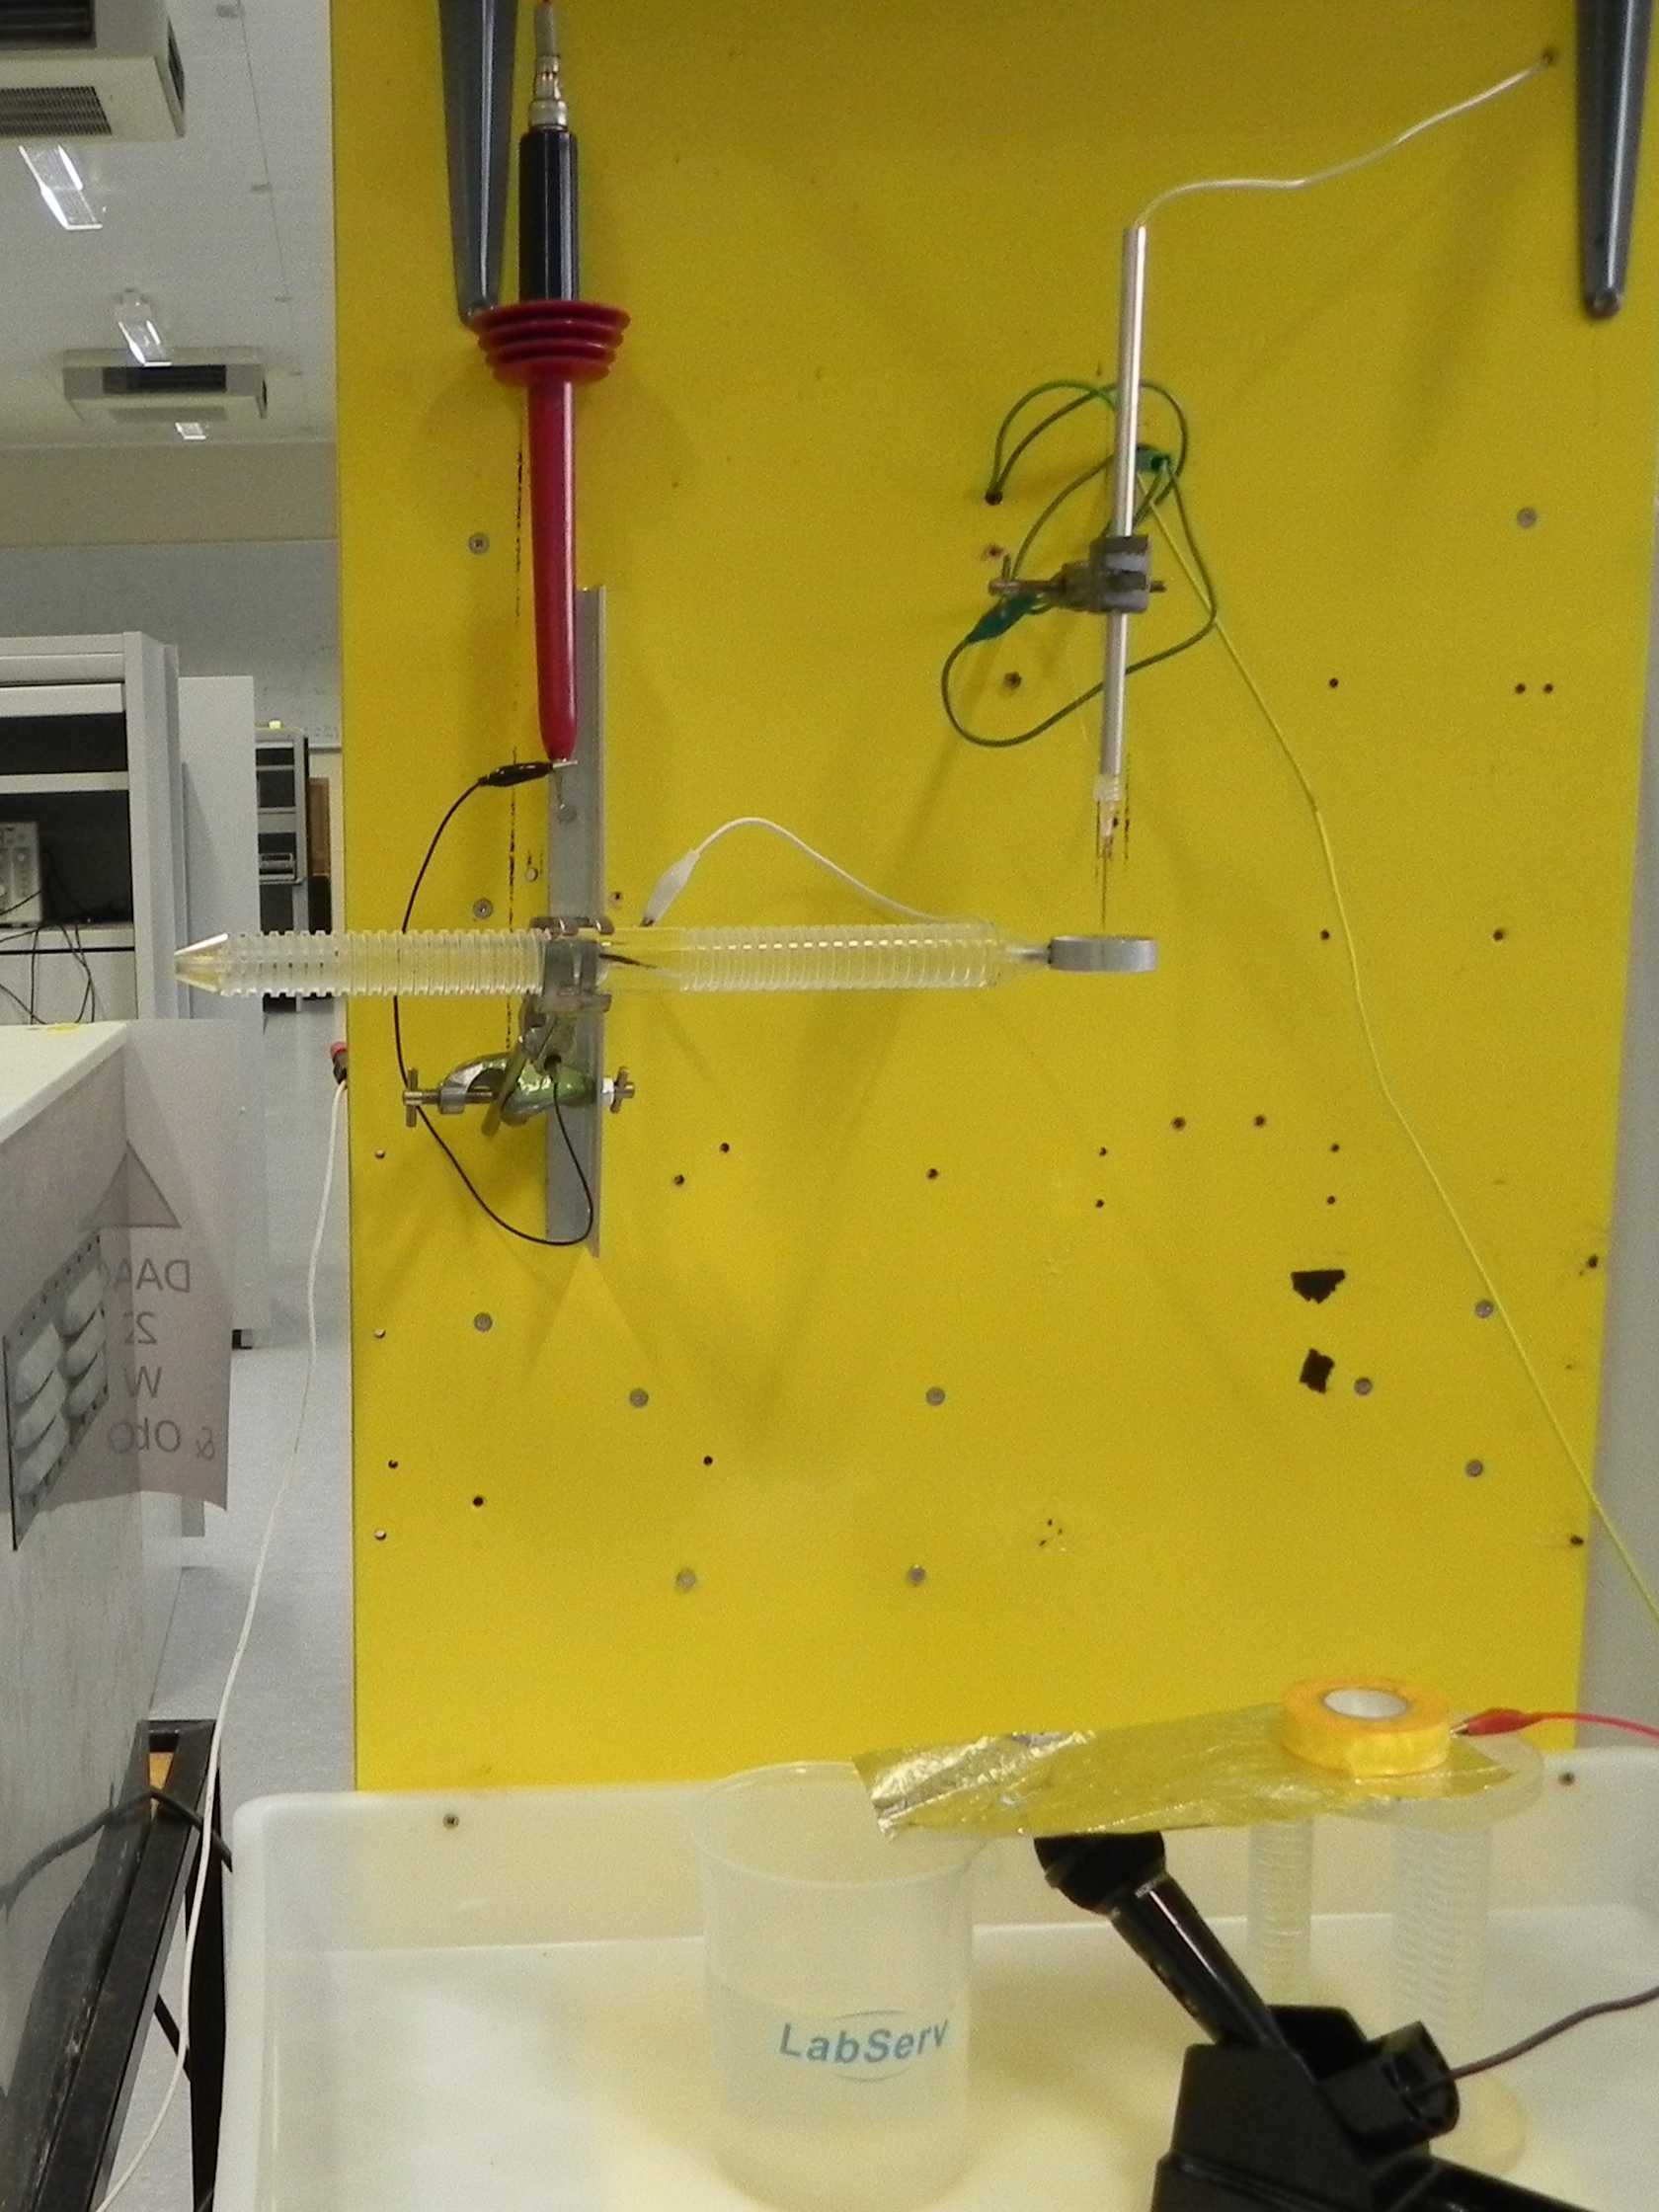
\includegraphics[scale=0.15]{content/appendices/chargedWaterDrops/graphics/Photo_dripperExperiment_Setup_draft.JPG}
        \caption{\label{Photo_dripperExperiment_Setup}Photo of experimental setup for charge on drip measurements.}
    \end{figure}

    \begin{figure}[ht]
        \centering
        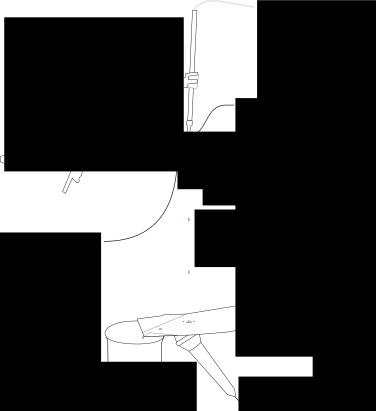
\includegraphics[scale=0.9]{content/appendices/chargedWaterDrops/graphics/ChargedDrips_Figure_Drawing_ExperimentalSetup}
        \caption{\label{ChargedDrips_Figure_Drawing_ExperimentalSetup}Diagram of experimental setup for charge on drip experiments.}
    \end{figure}

    \begin{figure}[ht]
        \centering
        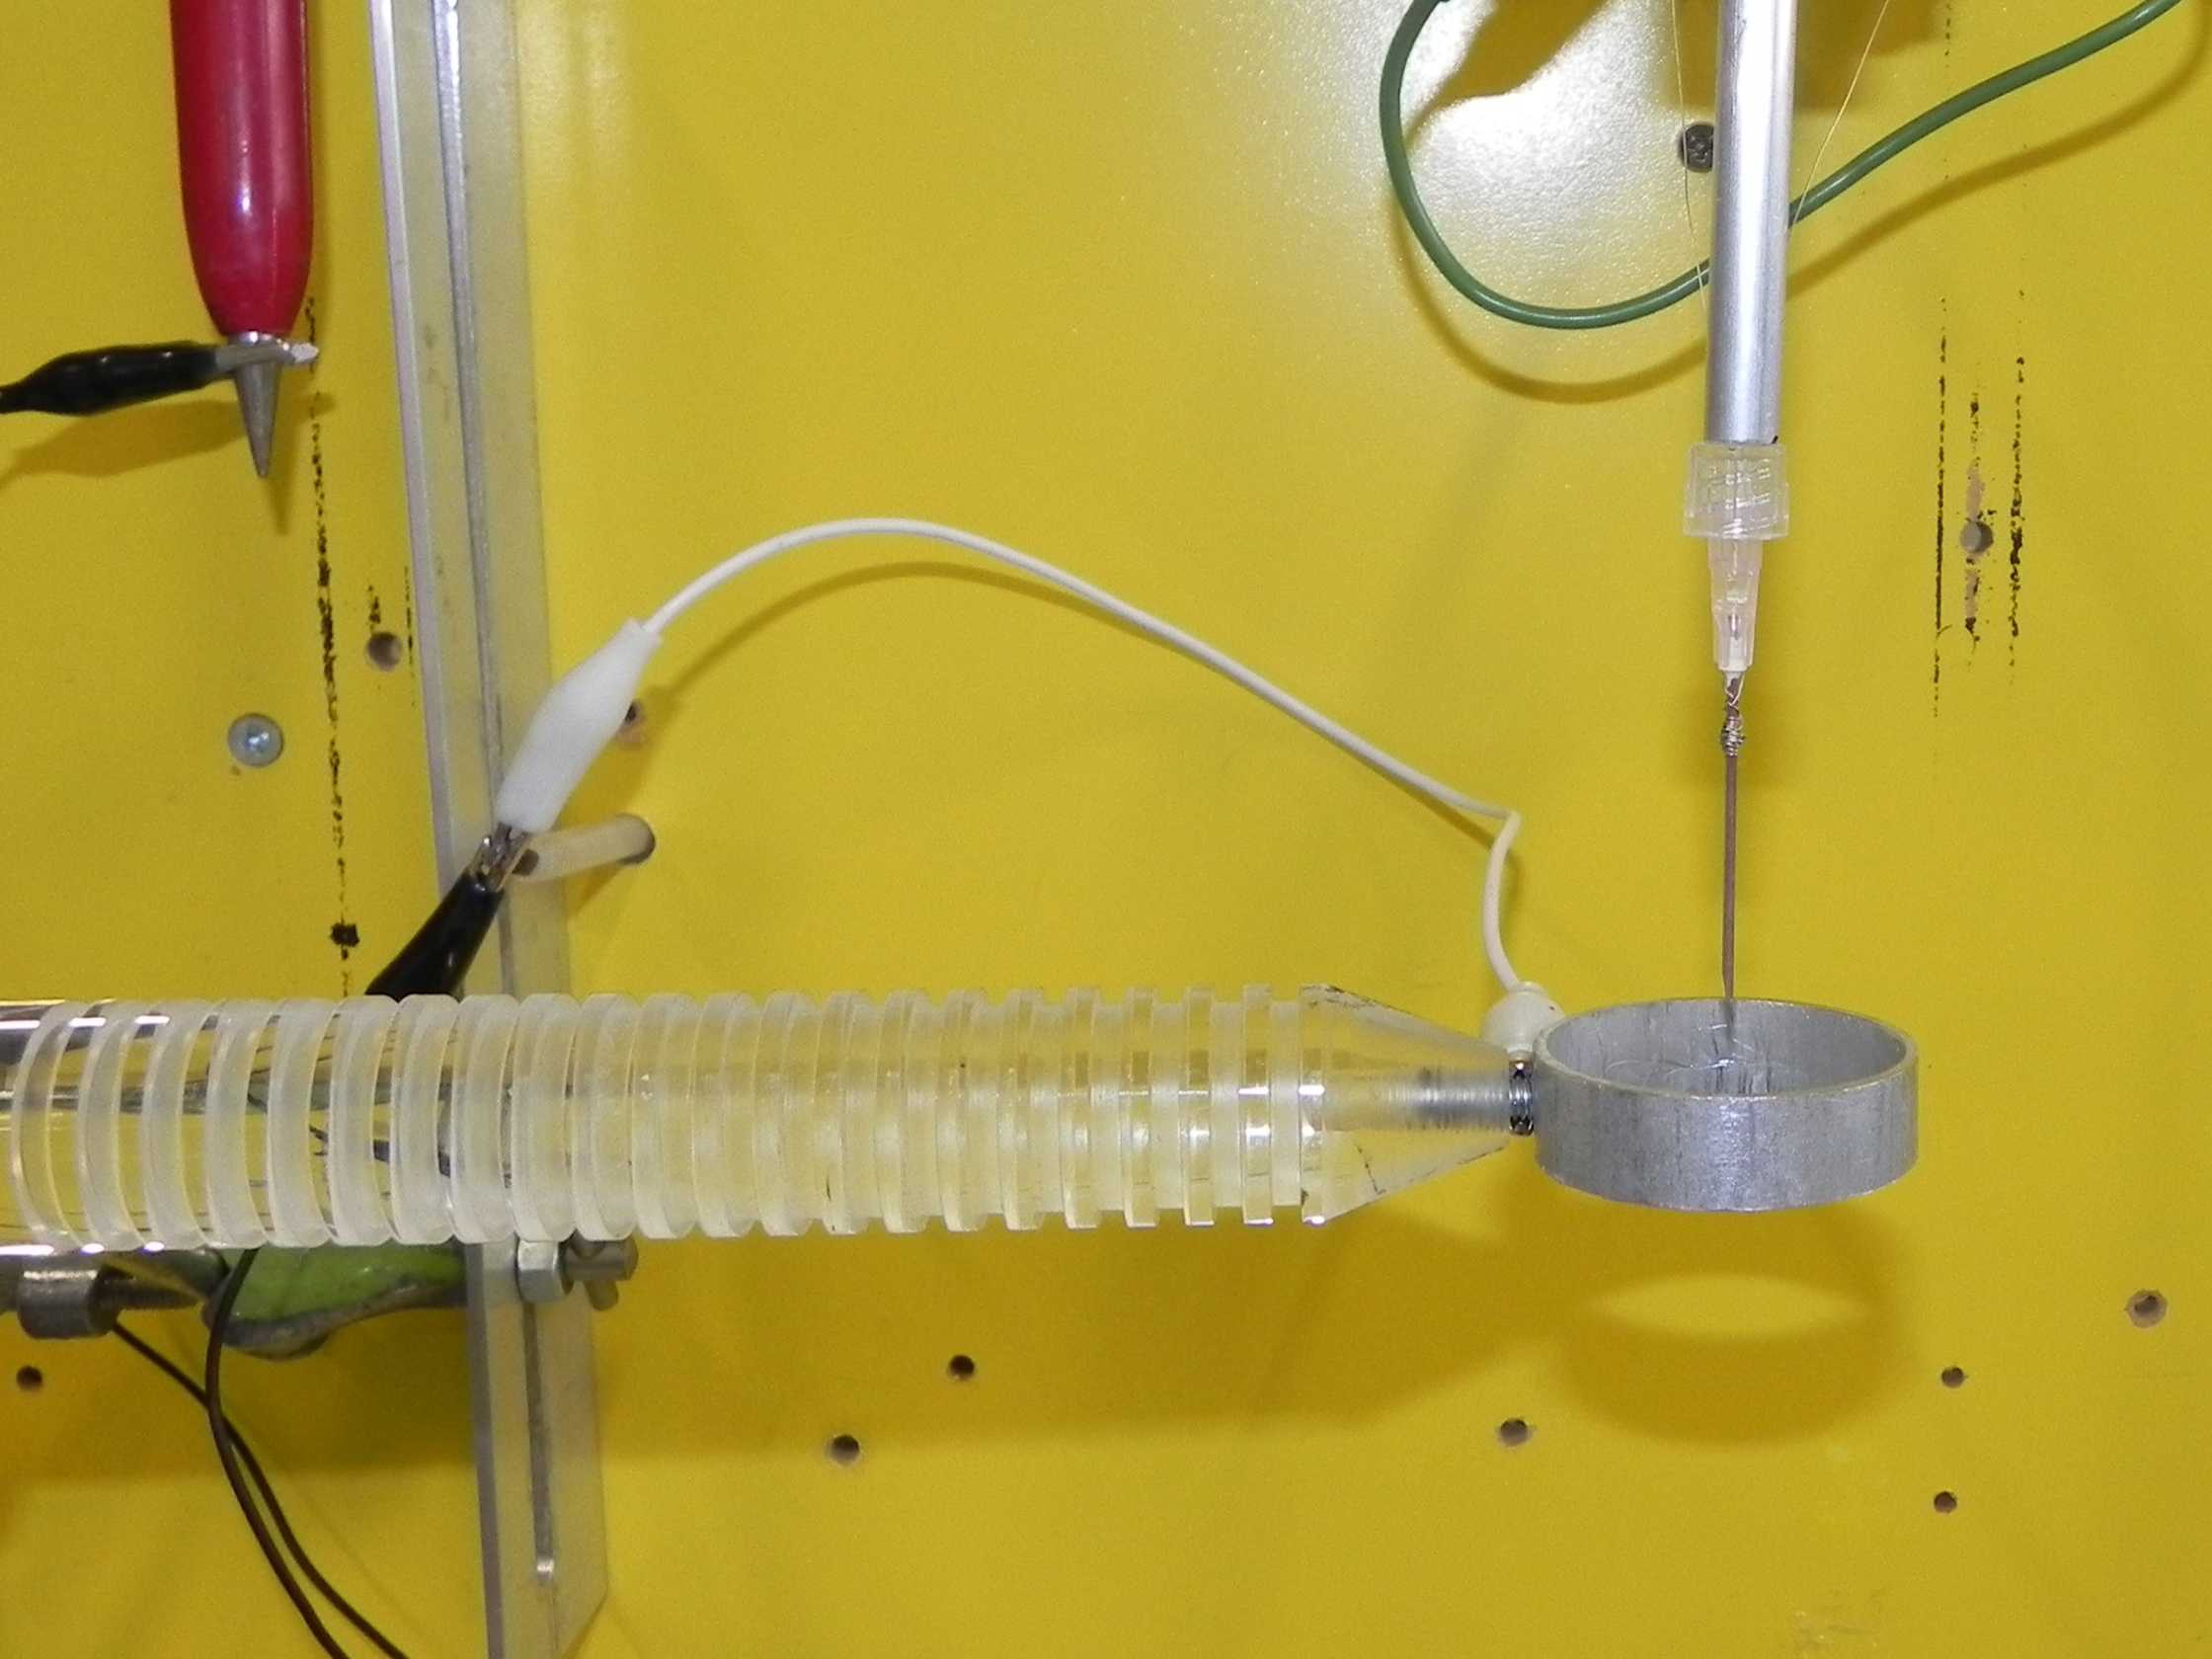
\includegraphics[scale=0.12]{content/appendices/chargedWaterDrops/graphics/Photo_dripperExperiment_Inductor_draft.JPG}
        \caption{Photo of the dropper and high voltage inductor.}
        \label{Photo_dripperExperiment_Inductor}
    \end{figure}

    \begin{figure}[ht]
        \centering
        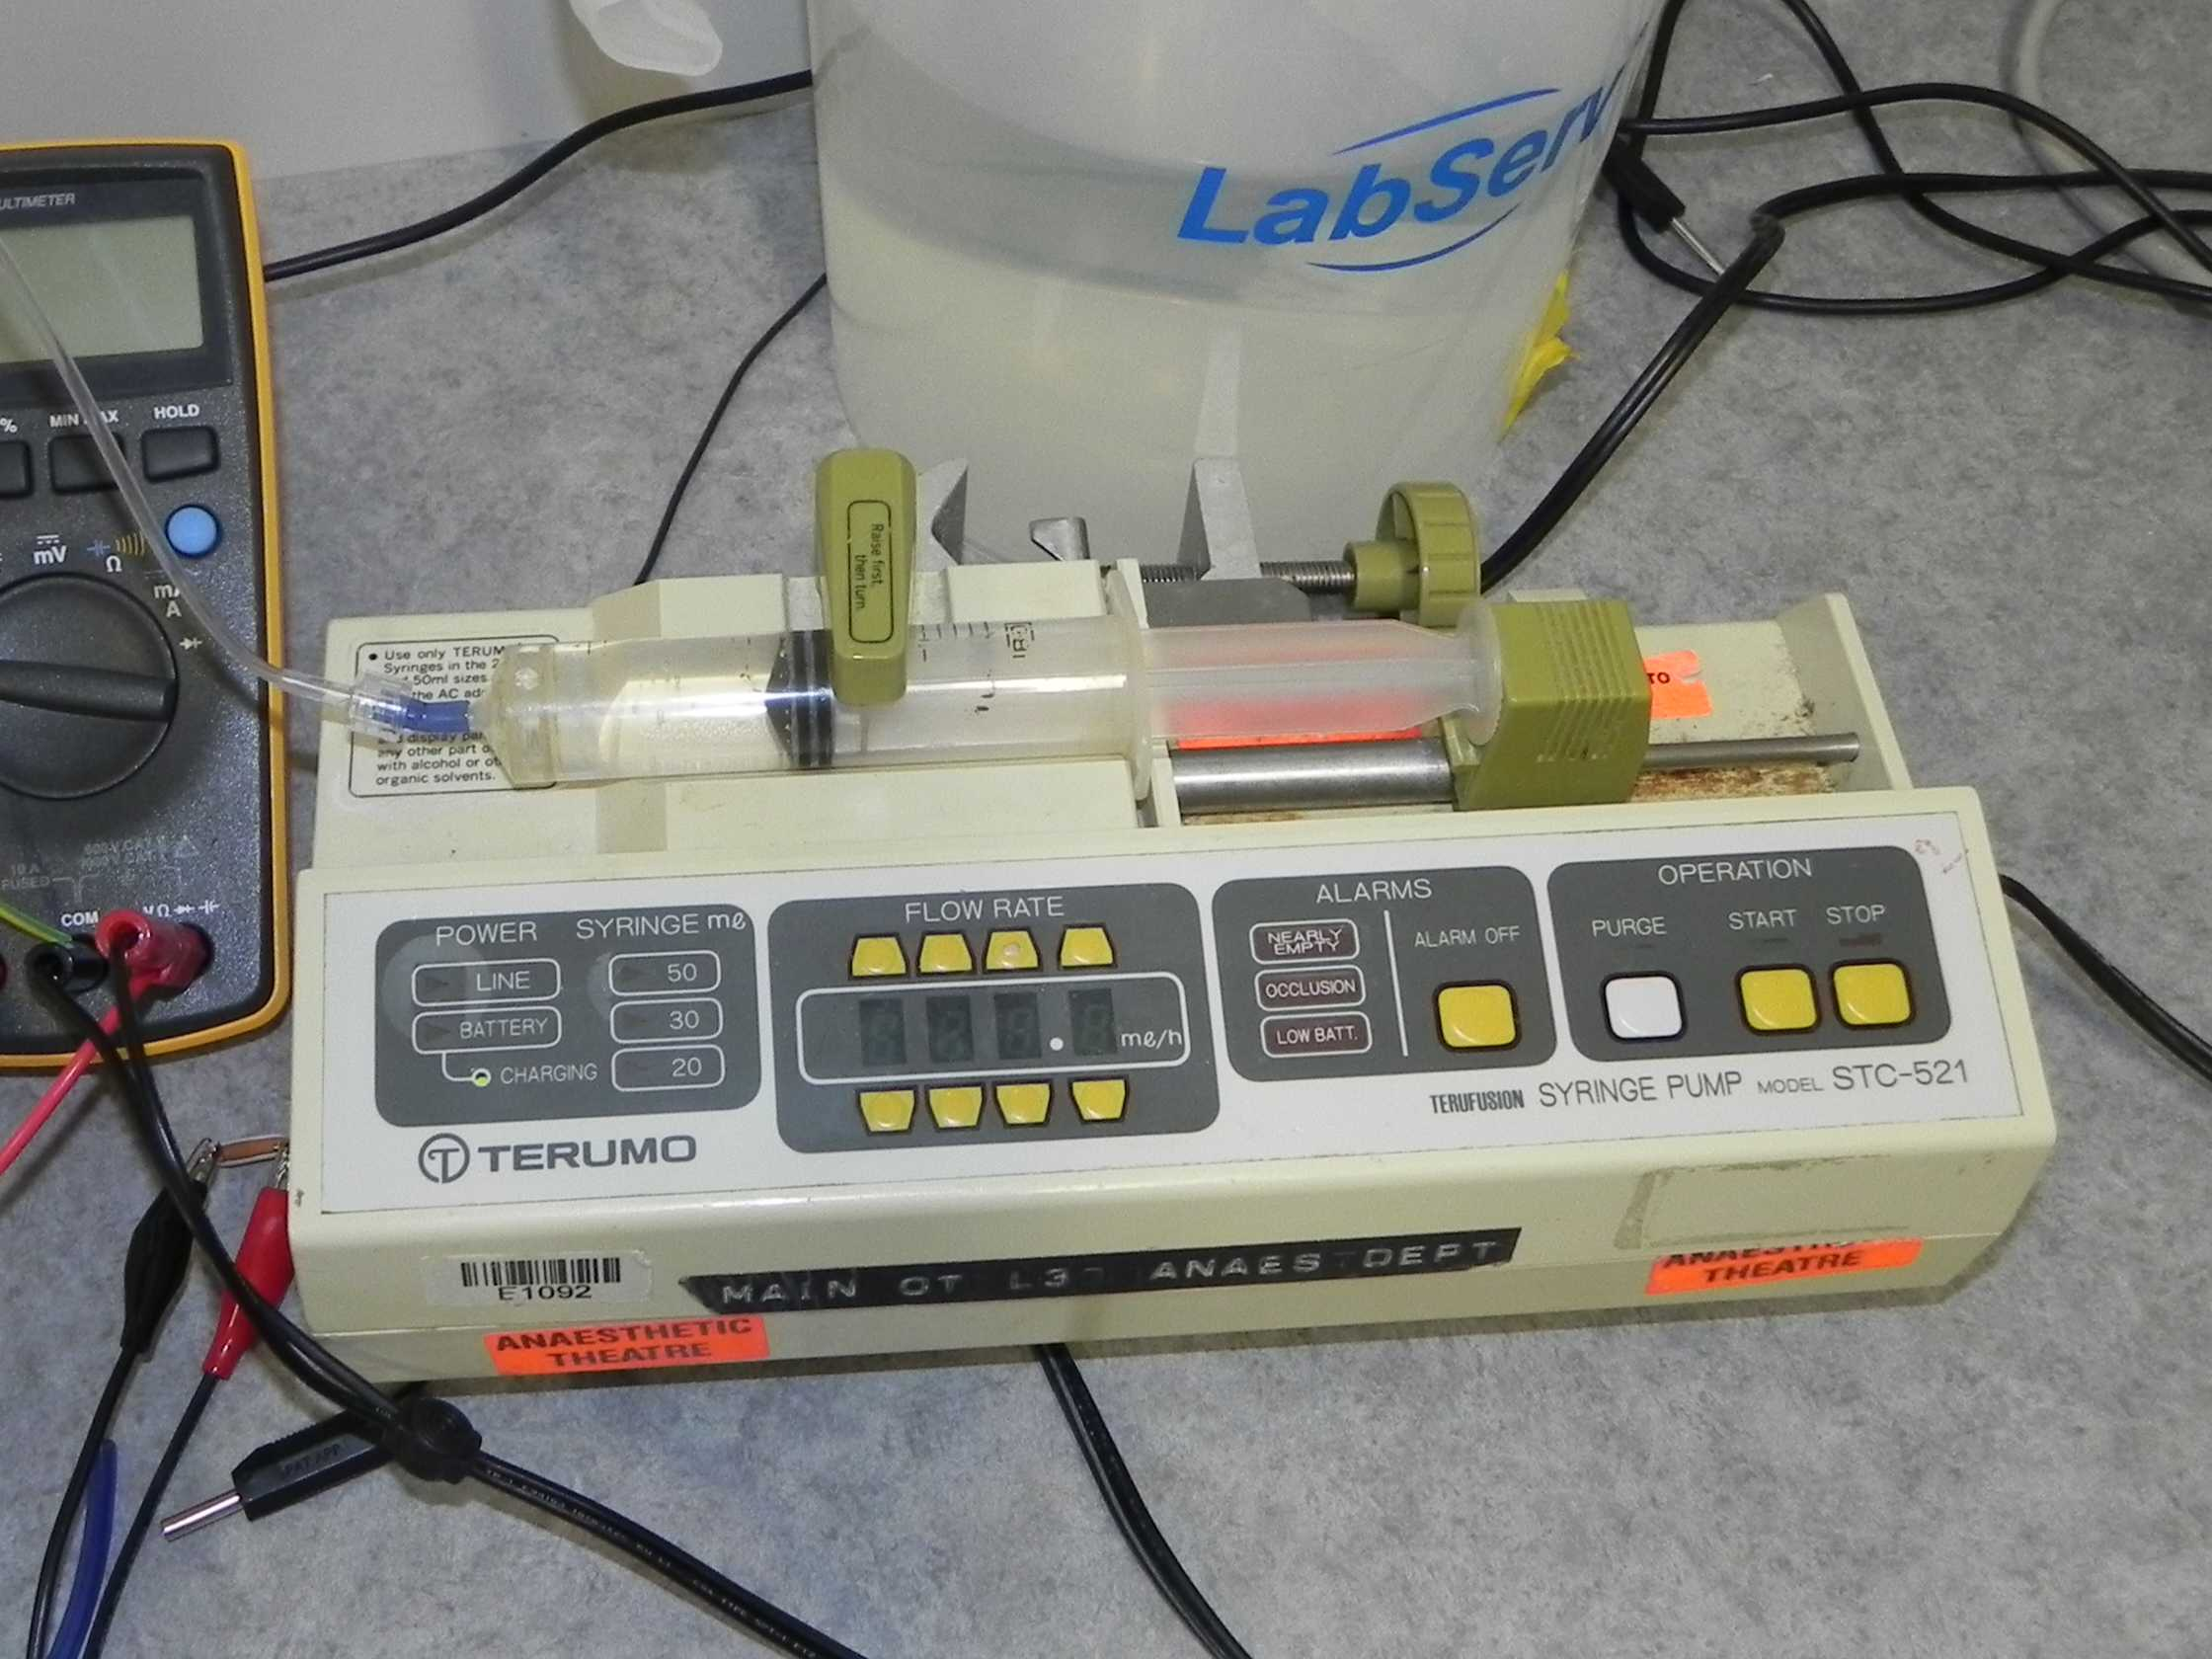
\includegraphics[scale=0.15]{content/appendices/chargedWaterDrops/graphics/Photo_dripperExperiment_SyringePump_draft.JPG}
        \caption{\label{Photo_dripperExperiment_SyringePump}Photo of the syringe pump used to produce drops and control flow rate.}
    \end{figure}

    A photo of the measurement setup is shown in \cref{Photo_dripperExperiment_Setup}.
    A simplified diagram of that same setup is shown in \cref{ChargedDrips_Figure_Drawing_ExperimentalSetup}.
    Drips are formed from a syringe needle which then fall through the induction ring before hitting the tin foil.
    A close-up of photo of the needle and inductor is shown in \cref{Photo_dripperExperiment_Inductor}.
    The drips frequency is determined by a microphone paced under the foil and the flow of water is set by the syringe pump (shown in \cref{Photo_dripperExperiment_SyringePump}).
    The volume of each drip is calculated by dividing the flow rate by the drip frequency.
    The charge on each drop is determined by dividing the average current through the multimeter by the drip frequency.
    Measured current was in the nano Ampere range so direct current measurement with a multimeter was not possible.
    Instead, the multimeter was set to measure voltage and the internal resistance of the meter itself was used as the current sense resistor.
    The multimeter had an internal resistance of \SI{10}{\mega\ohm}.
%    Ohms law states:
%    \begin{equation}
%    V=IR
%    \end{equation}
%    Where V is voltage, I is current and R is resistance.
%    Rearranging this equation and substituting in our resistance of \SI{10}{\mega\ohm} gives:
%
%    \begin{equation}
%    I=\frac{V}{10\times10^{6}}
%    \end{equation}
%    Where V is the output of the multimeter and I is the current through
%    the multimeter, through which we assume all charge collected on the
%    tin foil will flow.

  \subsubsection*{Results}

    \begin{figure}
        \centering
        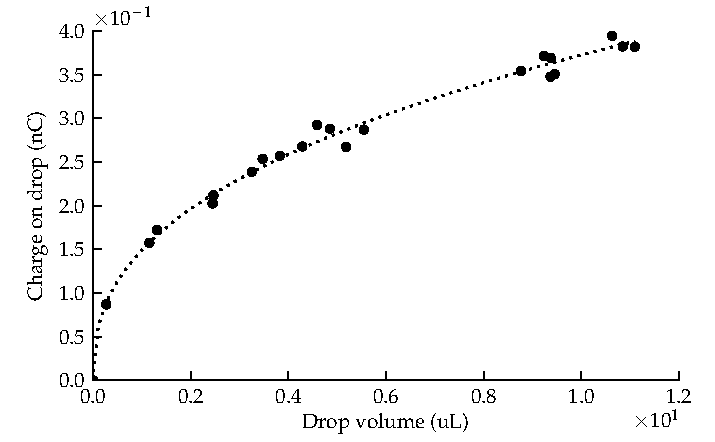
\includegraphics{content/appendices/chargedWaterDrops/graphics/dripper_chargeVsVolume}
        \caption{\label{Graph_dripperExperiment_chargeVsVolume}Charge on drip versus drip volume for a fixed induction voltage of \SI{2.5}{\kilo\volt}.}
    \end{figure}
    \begin{figure}
        \centering
        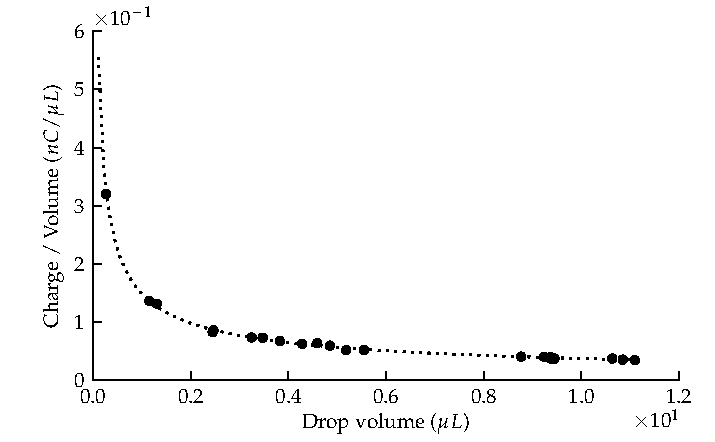
\includegraphics{content/appendices/chargedWaterDrops/graphics/dripper_chargePerVolumeVsVolume}
        \caption{\label{Figure_Graph_dripper_chargePerVolumeVsVolume}Charge per volume
        versus drop volume for a fixed induction voltage of \SI{2.5}{\kilo\volt}.}
    \end{figure}
    \begin{figure}
        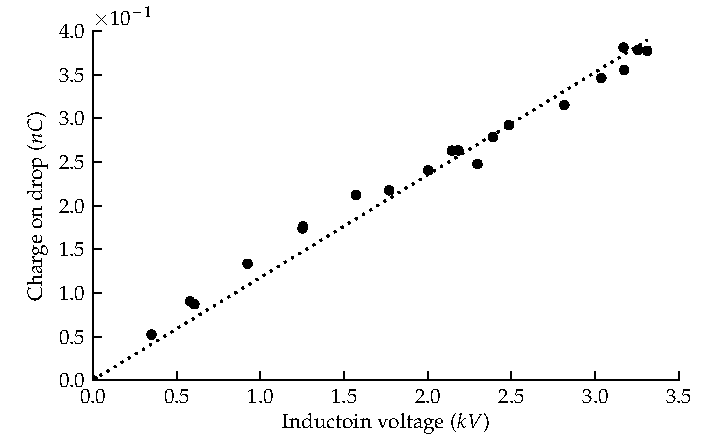
\includegraphics{content/appendices/chargedWaterDrops/graphics/dripper_chargeVsVoltage}
        \caption{\label{Figure_Graph_dripper_chargeVsVoltage}Graph showing charge on a drop versus induction voltage for a fixed drop volume.}
    \end{figure}
    Figure \ref{Figure_Graph_dripper_currentVsFlow} shows the effect of increasing the flow on the output current; a relatively linear response.
    \begin{figure}
        \centering
        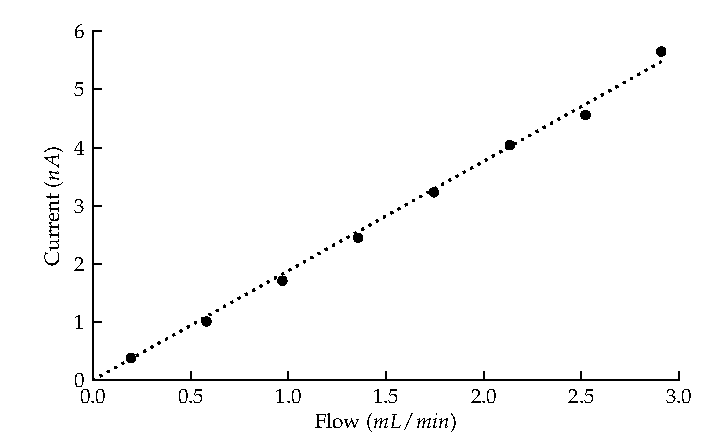
\includegraphics{content/appendices/chargedWaterDrops/graphics/dripper_currentVsFlow}
        \caption{\label{Figure_Graph_dripper_currentVsFlow}Graph showing current versus flow rate for an induction voltage of \SI{3.8}{\kilo\volt} and drop volume of \SI{3.1}{\micro\litre}.}
    \end{figure}
    Figure \ref{Graph_dripperExperiment_chargeVsVolume} shows the effect of drip volume on the bound charge per drop.
    This curve resembles the surface area of a sphere against the volume of a sphere.
    This was expected as excess charge will distribute itself over the outer surface of the drop, and therefore be proportional to its surface area.
    If the same data is plotted in terms of charge per volume versus volume of a drip, as is shown in Figure \ref{Figure_Graph_dripper_chargePerVolumeVsVolume}, it is evident that smaller drop sizes equate to a higher charge per volume of water ratio.
    Figure \ref{Figure_Graph_dripper_chargeVsVoltage} shows the results of changing the induction voltage on the average charge carried per drop.
    The results show the charge induced on a drop is proportional to the induction voltage.
    Variation in the measurement data is due to variations in room temperature.


  \subsubsection*{Conclusion \& discussion}

    Increasing the output of the generator is possible by:
    \begin{itemize}
    \item reducing the drop size for a given volumetric flow rate,
    \item increasing the volumetric flow rate,
    \item increasing the voltage on the induction ring.
    \end{itemize}
    Increasing the volumetric flow through a nozzle causes drops to turn into a stream above a flow threshold.
    If that stream does not break into drops before connecting with the receiving vessel then charge held in the vessel can travel up the stream; short-circuiting the device.
    If the stream does reliably break into droplets then the induction ring should be positioned as close to the transition point as possible.
    Reducing drop size and increasing the induction voltage both increase the charge to mass ratio of individual drops.
    As this ratio increases, the movement of drops becomes increasingly dominated by the electrostatic force between the receiver and the drop.
    The force repels the drop from the receiver meaning that the drops start to bend away from the receiver as the fall.
    Increasing the charge-to-mass ratio too far cause drops to escape the receiver.
    It is possible with a sufficiently large charge-to-mass ratio for the water droplets path to bend back upward to the induction ring, i.e., the water ``falls upwards'' back to the high voltage ring.
    A nozzle capable of producing consistent drop volumes allows for the greatest efficiency since the charge per drop can be maximised with the least reduction of drop catchment.

  \subsection*{Scale}

    Lord Kelvin's original design of electrostatic generator is too big to fit inside a water meter.
    Because of its size the voltage differential required to create the target electrostatic field strength is large; approximately \SI{4}{\kilo\volt}.
    A reduction in physical size would lower this voltage while keeping the electric field gradient the same.
    Notice in \cref{Photo_dripperExperiment_Inductor} how revolved cuts have been made in the arm supporting the induction ring to increase electrical isolation.
    Lower voltages would mean less electrical isolation is necessary keep the device from self-discharging.
    Reducing the scale of the device would allow it to generate a maximum output at voltages that are easier to process using conventional electronics.


%  \subsubsection*{Investigation:}
%
%    \begin{figure}
%        \centering
%        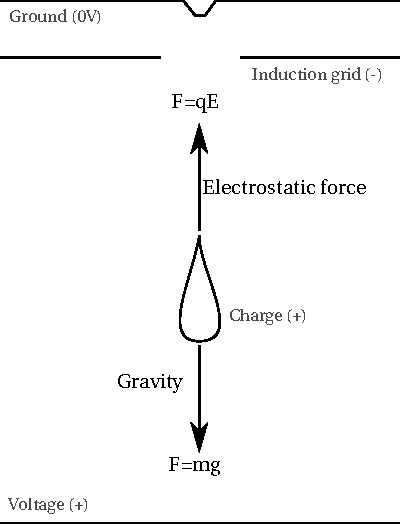
\includegraphics{content/appendices/chargedWaterDrops/graphics/ChargedDrips_Figure_Diagram_Forces}
%        \caption{\label{Figure_Diagram_ChargedDrips_Figure_Diagram_Forces}Diagram
%    of the electrostatic force and gravity acting on a drop of water.}
%    \end{figure}
%
%
%    Figure \ref{Figure_Diagram_ChargedDrips_Figure_Diagram_Forces} shows
%    a simplified diagram of the two dominant forces acting upon a charged
%    drop as it falls towards a like charged plate from a grounded plane.
%    These forces are given by the following equations:
%    \begin{equation}
%    F_{down}=mg
%    \end{equation}
%    \begin{equation}
%    F_{up}=qE
%    \end{equation}
%    where $m$ is the mass of the drop, $g$ is the acceleration due to
%    gravity, $q$ is the charge on the drop and $E$ is the electric field
%    strength.
